\documentclass[12pt, a4paper]{article}
\usepackage[utf8]{inputenc}
\usepackage[russian]{babel}
\usepackage[T2A]{fontenc}
\usepackage{amsfonts}
\usepackage{amsmath}
\usepackage{indentfirst}
\usepackage{amsthm}
\usepackage{algorithm,algpseudocode}
\DeclareMathOperator*{\minn}{min}
\DeclareMathOperator*{\argmin}{argmin}
\newtheorem{theorem}{Theorem}[section]
\newtheorem{state}{Утверждение}[section]
\newtheorem{lemma}{Лемма}[section]
\newtheorem{corollary}{Следствие}[section]


\usepackage[left=2cm,right=1.5cm,top=2cm,bottom=2cm]{geometry}
\linespread{1.25}

\usepackage{graphicx}
\graphicspath{{pictures/}}
\DeclareGraphicsExtensions{.pdf,.png,.jpg}

\begin{document}
\pagestyle{empty}

\begin{center}
	ФЕДЕРАЛЬНОЕ ГОСУДАРСТВЕННОЕ БЮДЖЕТНОЕ ОБРАЗОВАТЕЛЬНОЕ\\
	УЧРЕЖДЕНИЕ ВЫСШЕГО ОБРАЗОВАНИЯ\\
	<<МОСКОВСКИЙ ГОСУДАРСТВЕННЫЙ УНИВЕРСИТЕТ\\
	имени М.\,В.~ЛОМОНОСОВА>>
\end{center}
\vspace{4pt}
\begin{center}
	МЕХАНИКО-МАТЕМАТИЧЕСКИЙ ФАКУЛЬТЕТ
\end{center}
\vspace{4pt}
\begin{center}
	КАФЕДРА ВЫЧИСЛИТЕЛЬНОЙ МАТЕМАТИКИ
\end{center}
\vspace{1cm}
\begin{center}
	ВЫПУСКНАЯ КВАЛИФИКАЦИОННАЯ РАБОТА\\
	специалиста
\end{center}

\begin{center}
	\textbf{ОПТИМИЗАЦИЯ ТРАНСПОРТНОГО ПОТОКА \\
		    ПРИ ЗАДАННЫХ ПУНКТАХ ОТПРАВЛЕНИЯ И НАЗНАЧЕНИЯ \\
		    ВСЕХ УЧАСТНИКОВ ДВИЖЕНИЯ}
\end{center}
\vspace{1cm}
\begin{center}
	\begin{tabular}{p{9cm} l}
		& Выполнил студент $610$ группы\\
		& Пехтерев Станислав Игоревич\\
		& $\phantom{C_n^k=C_n^{n-k}}$\\
		& $\underline{\phantom{\int\limits_a^bf(x)dx=F(b)-F(a)}}$\\
		& подпись студента\\
		& $\phantom{\int\limits_f(z)dz=0}$\\
		& Научный руководитель:\\
		& доктор физико-математических наук \\
		& Васенин Валерий Александрович\\
		& $\phantom{C_n^k=C_n^{n-k}}$\\
		& $\underline{\phantom{\int\limits_a^bf(x)dx=F(b)-F(a)}}$\\
		& подпись научного руководителя\\
	\end{tabular}
\end{center}
\vspace{1cm}
\begin{center}
	Москва\\
	$2022$
\end{center}

\newpage
\pagestyle{plain}
\tableofcontents{}
\newpage	
	
 \section*{Тема}



\section{Введение}


\newpage
\section{Постановка задачи}

Для начала поставим общую задачу оптимизации транспортного потока.

%{Пусть задан граф $G = (V, E)$, описывающий некоторую \textit{дорожную сеть}. Предположим, что имеется $n$ участников движения по этому графу. Каждый участник $i$ имеет точки отправления $A_i \in V$ и точки прибытия $B_i \in V$. Пусть множество $P_i$ есть множество всех простых путей из $A_i$ в $B_i$. Пусть декартово произведение ${P = \prod \limits_{i = 1} ^ n P_i}$ есть множество всех возможных комбинаций путей участников. Элементы этого множества назовем \textit{комбинацией путей}. Пусть известно, что при комбинации путей участников ${\textbf{p} \in P}$ $i$-ый участник затрачивает $T_i(\textbf{p})$ времени на передвижение. }

\subsection{Общая постановка задачи}

Пусть задан ориентированный граф $G = (V, E)$, описывающий некоторую \textit{дорожную сеть}. Предположим, что имеется $n$ участников движения по этому графу. Каждый участник $i$ имеет точки отправления $A_i \in V$ и точки прибытия $B_i \in V$. Пусть множество $P_i$ есть множество всех простых путей из $A_i$ в $B_i$. Пусть декартово произведение ${P = \prod \limits_{i = 1} ^ n P_i}$ есть множество всех возможных комбинаций путей участников. Элементы этого множества назовем \textit{комбинацией путей}. Пусть известно, что при комбинации путей участников ${\textbf{p} \in P}$ $i$-ый участник затрачивает $T_i(\textbf{p}) \in \mathbb{R}$ времени на путь. 
Функции  $T_i$ назовем \textit{функциями временных затрат} участника $i$.
\textit{Некооперативным прокладыванием пути в ориентированном графе G} назовем пятерку $F = (n, G, \{A_i\}_{i = 1}^{n}, \{B_i\}_{i = 1}^{n}, \{T_i\}_{i = 1}^{n})$. Некооперативное прокладывание пути предпологает, что каждый участник стремится сократить собственные временные затраты путем выбора пути $\textbf{p}_i$, невзирая на временные затраты других участников. 
Для того чтобы скооперировать участников, введем некоторую функцию $\Phi (\textbf{p}) = \phi (T_1 (\textbf{p}), \ldots, T_n(\textbf{p}))$, определенную на множестве всех возможных комбинацией путей $P$ и отображающая его в множество действительных чисел, посредством которой они могут отслеживать как влияет изменение их пути на общую картину движения. Такую функцию назовем \textit{функцией стоимости}.

Для заданного некооперативного прокладвания пути $F$ и функции стоимости $\Phi$ необходимо найти такую комбинацию путей $\textbf{p}^*$, что функция стоимости минимальна на ней, то есть

\begin{equation}
	\label{eq:target_global_task_T} 
	\Phi (\textbf{p}^*) = \minn\limits_{ \textbf{p} \in P} \Phi (\textbf{p}).
\end{equation}

Комбинацию путей $\textbf{p}^*$ будем называть \textit {оптимальной}, а стоимость  $ \Phi (\textbf{p}^*)$ \textit {оптимальной стоимостью}.

Далее будем считать, что каждый участник имеет одинаковый приоритет в вопросе изменения своих временных затрат, то есть 

\begin{equation}
	\frac{\partial \phi}{\partial T_i} \equiv 1, \text{ } i = 1, \ldots, n,
\end{equation}

или, 

\begin{equation}
\phi(T_1, \ldots, T_n) = \sum\limits_{i = 1}^nT_i.
\end{equation}

\subsection{Постановка задачи в терминах модели движения}

Сложность численного решения задачи поиска оптимальной комбинации путей во многом зависит от аналитического задания функций $T_i (\textbf{p})$. Далее приведем ряд ограничений на функции $T_i (\textbf{p})$ нашей задачи, которую собираемся исследовать.

Будем считать, что на временные затраты при проезде по пути $\textbf{p}_i$ в первую очередь влияют временные затраты на ребрах, составляющих маршрут $\textbf{p}_i$. Поэтому без ограничения общности считаем, что функции временных затрат есть суммарные временные затраты на каждом ребре этого пути.

$$T_i (\textbf{p}) = \sum \limits_{e \in E} \overline{\tau}_{e, i} (\textbf{p}) = \sum \limits_{e \in \textbf{p}_i} \overline{\tau}_{e, i} (\textbf{p}), $$

где функции $\overline{\tau}_{e, i} (\textbf{p})$ есть временные затраты $i$-ого участника на ребре $e$ при комбинации путей $\textbf{p}$. 

Будем рассматривать те некооперативные прокладывания пути, в которых существует движение каждого участника для каждой комбинации путей $\textbf{p}$, то есть в каждый момент времени $t \in \mathbb{R}$ известно положение участника на пути. Таким образом, будем считать, что для каждой комбинации путей $\textbf{p}$ и времени $t$ известно присутствует ли участник $i$ на ребре $e$, то есть известны функции

$$
\theta_{e, i} (\textbf{p}, t) =
\begin{cases}
	1, & \text{если }  i\text{-ый участник движется по ребру $e$ в момент времени $t$,}  \\
	0, & \text{иначе},
\end{cases}
$$

где $\sum\limits_{e \in E} \theta_{e, i} (\textbf{p}, t)$ принимает значение $1$ пока участник не доедет до своей точки назначения $B_i$, и $0$ после. Также будем считать, что достижение  участником $i$ вершины $B_i$ наступает в момент $T_i(\textbf{p})$, то есть 
	
\begin{equation}
	\label{eq:T_i_by_theta}
	T_i(\textbf{p}) = \sum \limits_{e \in \textbf{p}_i} \int\limits_{0}^{T_i(\textbf{p}) + \Delta t} \theta_{e, i} (\textbf{p}, t) dt, \forall \Delta t > 0.
\end{equation}

Будем считать, что передвижение каждого учаcтника является непрерывным и последовательным относительно графа $G$. Другими словами участник не может резко повлятся и исчезать на несмежных ребрах, а также посещать пройденные ребра. Таким образом считаем, что функции $\theta_{e, i} (\textbf{p}, t)$ являются индикаторами некоторых интервалов $[t_{e, i}^{in} (\textbf{p}), t_{e, i}^{out} (\textbf{p})]$, которые описывают последовательное передвижение:

\begin{equation}
	\label{eq:restr_t}
	\begin{cases}
		t_{e, i}^{in}(\textbf{p}), t_{e, i}^{out}(\textbf{p}) \in \mathbb{R}_+,  & i = 1, \dots, n, \text{ } e \in E, \\
		t_{e, i}^{in}(\textbf{p}) \le t_{e, i}^{out}(\textbf{p}), & i = 1, \dots, n, \text{ } e \in \textbf{p}_i,  \\
		t_{e, i}^{in}(\textbf{p}) = t_{e, i}^{out}(\textbf{p}) = 0, & i = 1, \dots, n, \text{ } e \notin \textbf{p}_i, \\
		t_{e_1, i}^{in} (\textbf{p}) = t_{e_2, i}^{out} (\textbf{p}), & i = 1, \dots, n, \text{ } e_1, e_2 \in \textbf{p}_i, \exists A, B, C \in V: e_1 = (A, B), e_2 = (B, C)\\
		t_{e, i}^{in} (\textbf{p}) = 0, & i = 1, \dots, n, \text{ } e = (A_i, X), X \in V.
	\end{cases}
\end{equation}

Заметим, что выбор таких интервалов пока неоднозначен. Далее считаем, что для каждого ребра $e$, участника $i$ и комбинации путей $\textbf{p}$ каким-то образом выбраны некоторые велечины $t_{e, i}^{in}(\textbf{p}), t_{e, i}^{out}(\textbf{p})$, удовлетворяющие ограничениям \eqref{eq:restr_t}. Тогда функция временных затрат \eqref{eq:T_i_by_theta} $i$-ого участника примет вид

\begin{equation}
	\label{eq:T_i_by_t}
	T_i(\textbf{p}) = \sum \limits_{e \in E} t_{e, i}^{out}(\textbf{p}) - t_{e, i}^{in}(\textbf{p}).
\end{equation}

Функция стоимости в этом случае есть 

\begin{equation}
	\label{eq:target_func}
	\Phi(\textbf{p}) =\sum \limits_{i = 1}^n \sum \limits_{e \in E} t_{e, i}^{out}(\textbf{p}) - t_{e, i}^{in}(\textbf{p}).
\end{equation}

Без ограничения общности считаем, что временные затраты участником $i$ на ребре $e$ ограничены некоторыми положительными константами $\overline{\tau}_{e, i}^{min}, \overline{\tau}_{e, i}^{max}$:

\begin{equation}
	\label{eq:add_restr}
		0 < \overline{\tau}_{e, i}^{min} \le t_{e, i}^{out}(\textbf{p}) - t_{e, i}^{in}(\textbf{p}) \le \overline{\tau}_{e, i}^{max}, e \in \textbf{p}_i,\, i = 1, \dots, n,
\end{equation}

Заметим, что задача оптимизации с целевой функцией \eqref{eq:target_func} и ограничениями \eqref{eq:restr_t}, \eqref{eq:add_restr} ставится в терминах задачи смешанного целочисленного линейного программирования с вещественными переменными $t_{e, i}^{in}, t_{e, i}^{out} \in \mathbb{R}_+$, отвечающими за моменты прохождения $i$-ым участником ребра $e$ и булевыми переменными $I_{e, i} \in \{0, 1\}$, отвечающими за проезд по ребру $e$ участником $i$. Однако в данных ограничениях решение уже имеется --- участник $i$ передвигается по кратчайшему пути в графе $G$ с весами $\overline{\tau}_{e, i}^{min}$. Тревиальность решения связана с тем, что в данной задаче оптимизации отсутвутют влияния участников друг на друга. Для того, чтобы учесть это влияние, для каждого участника $i$ введем микроскопическую характеристику движения $v_i(\textbf{p}, t)$ ~--- положительная, ограниченная функция, описывающую скорость участника.


Тогда, имеет место следующее ограничение

\begin{equation}
	\label{eq:velocity_eq_by_theta}
	\int\limits_{0}^{T_i(\textbf{p})} \theta_{e, i} (\textbf{p}, t) v_i(\textbf{p}, t) dt = l_e, e \in \textbf{p}_i, i = 1, \dots, n,
\end{equation}

или,

\begin{equation}
	\label{eq:velocity_eq_by_t}
	\int\limits_{t_{e, i}^{in}(\textbf{p})}^{t_{e, i}^{out}(\textbf{p})} v_i(\textbf{p}, t) dt = l_e, e \in \textbf{p}_i, i = 1, \dots, n,
\end{equation}

где $l_e$~--- длина ребра $e \in E$. Будем говорить, что уравнения \eqref{eq:velocity_eq_by_t} задают \textit{модель движения участников}. Без ограничения общности считаем, что $\overline{\tau}_{e, i}^{min}, \overline{\tau}_{e, i}^{max}$ вычисляются в самом быстром и самом медленном варианте передвижения по ребру $e$ участником $i$, а именно

\begin{equation}
	\label{eq:restr_add_concrete}
	\overline{\tau}_{e, i}^{min} = \frac{l_e}{\max\limits_{\textbf{p} \in P, t \in \mathbb{R}} \left(  v_i(\textbf{p}, t) \right)}, \overline{\tau}_{e, i}^{max} = \frac{l_e}{\min\limits_{\textbf{p} \in P, t \in \mathbb{R}} \left(  v_i(\textbf{p}, t) \right)}
\end{equation}

Заметим, что велечины $t_{e, i}^{in}(\textbf{p}), t_{e, i}^{out}(\textbf{p}) \in \mathbb{R}_+$ - произвольные вещественные велечины, которые удовлетворяют ограничениям \eqref{eq:restr_t}, \eqref{eq:add_restr}, \eqref{eq:velocity_eq_by_t}, \eqref{eq:restr_add_concrete}.

\begin{state}
\label{state:modeling}
Пусть задан ориентированный граф $G$ и для каждого ребра $e$, участника $i$ и комбинации путей $\textbf{p}$ задано множество велечин $t_{e, i}^{in}(\textbf{p}), t_{e, i}^{out}(\textbf{p}) \in \mathbb{R}_+$, для которых выполняются ограничения \eqref{eq:restr_t}, \eqref{eq:add_restr}, \eqref{eq:velocity_eq_by_t}, \eqref{eq:restr_add_concrete}. Тогда $t_{e, i}^{out}(\textbf{p})$ и $t_{e, i}^{in}(\textbf{p})$, $e \in \textbf{p}_i$ есть функции от комбинации путей $\textbf{p} \in P$.
\end{state}
\begin{proof}
Зафиксируем некоторую комбинацию путей $\textbf{p}$. Опишем алгоритм поиска значений $t_{e, i}^{out}(\textbf{p})$ и $t_{e, i}^{in}(\textbf{p})$ и покажем его корректность.

\begin{algorithm}
	\caption{Моделирование движения участников}
	\label{alg:modeling}
	{\bf {Input:}} количество участников $n$, ориентированный граф $G$, комбинация путей $\textbf{p}$ графа $G$\\
	{\bf {Output:}} $t_{e, i}^{out}(\textbf{p})$, $t_{e, i}^{in}(\textbf{p})$, $e \in \textbf{p}_i, i = 1, \ldots, n$\\
	{\bf {Data:}} текущее время $t$, текущее ребро $e_i$ и часть пройденного ребра $x_i$ участника $i$
	\begin{algorithmic}[1]
		\State $t = 0$
		\For{$i = 1, \ldots, n$}
		\State $e_i \gets$ { первое ребро пути $\textbf{p}_i$}
		\State $x_i \gets 0$
		\State $t_{e_i, i}^{in}(\textbf{p}) \gets 0$ 
		\EndFor
		\While{$\exists i: i \text { --- не доехал}$}
		\State $\tau^* \gets \argmin\{ \tau \in \mathbb{R}: \tau > t, \int\limits_{t}^{\tau} v_i(\textbf{p}, t) dt = (1 - x_i) l_{e_i}, i \text{--- не доехал}  \}_{i = 1}^n$
		\For{$i = 1, \ldots, n$ \textbf{and} $i - \text{ не доехал}$ }
		\State $x_i \gets x_i + \frac{1}{l_{e_i}} \int\limits_{t}^{\tau^*} v_i(\textbf{p}, t) dt$
			\If{$x_i = 1$ \textbf{and} $e_i$ - не последнее ребро пути $\textbf{p}_i$ }
				\State $x_i \gets 0$
				\State $t_{e_i, i}^{out}(\textbf{p}) \gets \tau^*$ 
				\State $e_i \gets$ следующее ребро за $e_i$ в пути $\textbf{p}_i$
				\State $t_{e_i, i}^{in}(\textbf{p}) \gets \tau^*$ 
			\EndIf
		\EndFor
		\State $t \gets \tau^*$
		\EndWhile
	\end{algorithmic}
\end{algorithm}

Описанный алгоритм называется \textit{моделированием движения}.

\textit{Корректность}. Корректность шага 8 алгоритма и достижимость шага 11 следует из того, что функция скорости ограничена снизу (см. ограничения \eqref{eq:add_restr}, \eqref{eq:restr_add_concrete}). Алгоритм сойдется, поскольку пути $\textbf{p}_i$ конечны.

\end{proof}
 Используя это утверждение, задача \eqref{eq:target_global_task_T} с учетом введенных ограничений \eqref{eq:restr_t}, \eqref{eq:T_i_by_t}, \eqref{eq:add_restr}, \eqref{eq:velocity_eq_by_t}, \eqref{eq:restr_add_concrete} формулируется следующим образом:

Пусть задано некооперативное прокладывание пути $F = (n, G, \{A_i\}_{i = 1}^{n}, \{B_i\}_{i = 1}^{n}, \{\sum \limits_{e \in E} t_{e, i}^{out}(\textbf{p}) - t_{e, i}^{in}(\textbf{p})\}_{i = 1}^{n})$ и модель движения $v_i(\textbf{p}, t)$, где функции $t_{e, i}^{in}(\textbf{p}), t_{e, i}^{out}(\textbf{p})$ получены путем моделирования с моделью движения $v_i(\textbf{p}, t)$. Требуется найти такую комбинацию путей $\textbf{p}$, что функция 

\begin{equation}
\label{eq:target_task_end}
\Phi(\textbf{p}) =\sum \limits_{i = 1}^n \sum \limits_{e \in E} t_{e, i}^{out}(\textbf{p}) - t_{e, i}^{in}(\textbf{p})
\end{equation}

минимальна.

Заметим, что в случае, когда условие \eqref{eq:velocity_eq_by_t} можно описать в терминах задачи удовлетворения ограничений, задача оптимизации \eqref{eq:target_task_end} может быть описана в терминах смешанного целочисленного линейного программирование и, как следствие, может быть решена стандартным решателем.

\newpage
\section{Модели движения}

Рассмотрим несколько видов моделей движений, которые в разной степени описывают влияние участников друг на друга.

\subsection{Макроскопические модели}

Предположим, что скорость участника зависит от некоторой общей для участников велечины. Например, от функции загруженности ребра

$$ n_{e}(\textbf{p}, t) = \sum\limits_{i = 1}^n\theta_{e, i}(\textbf{p}, t),$$
значение которой в момент времени $t$ соответствует количеству участников на ребре $e$ в этот момент при комбинации путей $\textbf{p}$. Предположим скорость участника зависит только от загруженности ребра, на котором он находится:

\begin{equation}
	\label{eq:velocity_eq_macro}
	 v_i(\textbf{p}, t) = \sum \limits _{e \in E} \theta_{e, i} (\textbf{p}, t) v (n_e (\textbf{p}, t)),  i = 1, \dots, n
\end{equation}

Такую модель движения в дальнейшем будем называть \textit{макроскопической}.
Например, естествено расмотреть модель $ v (n_e (\textbf{p}, t)) = \frac{v_{max}}{n_e (\textbf{p}, t)}$. В общем случае такая модель задается последовательностью значений  $\{v(k)\}_{k = 1}^n$.

\begin{lemma}
	\label{lemma:lt}
	Пусть даны вещественные переменные $a$, $b$ целочисленного программирования и известно, что существует константа $M > 0$ : $|a| < M$, $|b| < M$. Тогда можно добавить новую целочисленную переменную $\textbf{1} (\{a < b\}) \in \{0, 1\}$ такую, что
	
	\begin{equation*}
		\textbf{1} (\{a < b\}) = 
		\begin{cases}
			1,\, a < b,
			\\
			0,\, a \ge b.
		\end{cases}
	\end{equation*}

\end{lemma}

\begin{proof}
	Добавим в нашу задачу два неравенства:
	
	$$ 2M (\textbf{1} (\{a < b\}) - 1) < b - a \le 2M\textbf{1} (\{a < b\}) $$
	
	Очевидная проверка показывает, что неравенство выполняется для любых $a, b$.
	
	
\end{proof}

\begin{state}
	
	\label{state:lin_prog}
	
	Пусть модель движения $ v_i(\textbf{p}, t)$ макроскопическая. Тогда задача \eqref{eq:target_task_end} есть задача смешанного целочисленного линейного программирования.
\end{state}

\begin{proof}
	Докажем для случая $n = 2$. Для случаев $n \ge 2$ доказательство аналогичное.
	
	Пусть имеется задача смешанного целочисленного линейного программирования \eqref{eq:restr_t} с переменными $t_{e, i}^{in}, t_{e, i}^{out}, I_{e, i}, e \in E, i = 1, 2$. Преобразуем условие \eqref{eq:velocity_eq_by_t} к каноническому виду задачи удовлетворения ограничений. Для удобства обозначим обоих участников индексами $i, j \in \{1, 2\}$.
	
	$$\int\limits_{0}^{\infty} \theta_{e, i} (\textbf{p}, t) v_i(\textbf{p}, t)dt = \int\limits_{0}^{\infty} \theta_{e, i} (\textbf{p}, t) \sum \limits _{e^1 \in E} \theta_{e^1, i} (\textbf{p}, t) v (n_{e^1} (\textbf{p}, t)) dt = $$
	
	$$\int\limits_{0}^{\infty} \theta_{e, i} (\textbf{p}, t)  v (n_{e} (\textbf{p}, t)) dt = 
	  \int\limits_{ \substack{n_{e} (\textbf{p}, t) = 1}} \theta_{e, i} (\textbf{p}, t)  v (n_{e} (\textbf{p}, t)) dt +
	  \int\limits_{ \substack{n_{e} (\textbf{p}, t) = 2}} \theta_{e, i} (\textbf{p}, t)  v (n_{e} (\textbf{p}, t)) dt = $$
	
	$$\int\limits_{ \substack{\theta_{e, j} (\textbf{p}, t) = 0}} \theta_{e, i} (\textbf{p}, t)  v (1) dt +
	  \int\limits_{ \substack{\theta_{e, j} (\textbf{p}, t) = 1}} \theta_{e, i} (\textbf{p}, t)  v (2) dt = $$
	  
    $$\int\limits_{0}^{\infty} \theta_{e, i} (\textbf{p}, t)  v (1) dt - 
      \int\limits_{ \substack{\theta_{e, j} (\textbf{p}, t) = 1}} \theta_{e, i} (\textbf{p}, t)  v (1) dt +
	  \int\limits_{ \substack{\theta_{e, j} (\textbf{p}, t) = 1}} \theta_{e, i} (\textbf{p}, t)  v (2) dt = $$
	  
	$$v (1) \int\limits_{0}^{\infty} \theta_{e, i} (\textbf{p}, t) dt +
	  (v (2) - v(1)) \int\limits_{0}^{\infty} \theta_{e, i} (\textbf{p}, t) \theta_{e, j} (\textbf{p}, t) dt = $$
	  
    $$v (1) \overline{\tau}_{e, i} (\textbf{p}) +
    (v (2) - v(1)) \int\limits_{0}^{\infty} \theta_{e, i} (\textbf{p}, t) \theta_{e, j} (\textbf{p}, t) dt = l_e, e \in \textbf{p}_i$$
	  
	Неизвестный интеграл - время совместного проезда участников на ребре $e$.
	  
	В переменных задачи смешанного целочисленного программирования получим:
	
	$$v(1) (t_{e, i}^{out} - t_{e, i}^{in}) + (v(2) - v(1)) (t_{e, ij}^{out} - t_{e, ij}^{in}) = l_e I_{e, i},$$
	
	где новые перемнные $t_{e, ij}^{in}$, $t_{e, ij}^{out}$ отвечают за начало и конец совместного проезда участников. Другими словами $[t_{e, ij}^{in}, t_{e, ij}^{out}] = [t_{e, i}^{in}, t_{e, i}^{out}] \cap [t_{e, j}^{in}, t_{e, j}^{out}]$. Просуммировав по всем ребрам $e \in E$, получим
	
	$$v(1) \sum \limits _{e \in E} (t_{e, i}^{out} - t_{e, i}^{in}) = \sum \limits _{e \in E} l_e I_{e, i} - (v(2) - v(1)) \sum \limits _{e \in E} (t_{e, ij}^{out} - t_{e, ij}^{in})$$
	
	Заметим, что левая часть есть временные затраты участника $i$ с коэффициентом $v(1)$, поэтому задачу оптимизации можно переписать в виде
	$$ \frac{1}{v (1)} \sum\limits_{i = 1}^n \sum \limits _{e \in E} l_e I_{e, i} + \frac{v(1) - v(2)}{v (1)}  \sum\limits_{i = 1}^n \sum \limits _{e \in E} (t_{e, ij}^{out} - t_{e, ij}^{in}) \rightarrow \minn $$
	
	Для завершения доказательства необходимо показать, что переменные $t_{e, ij}^{in}, t_{e, ij}^{out}$ описываются линейными ограничениями. Обозначим $\Delta t = t_{e, ij}^{out} - t_{e, ij}^{in}, \Delta t_1 =  t_{e, i}^{out} - t_{e, i}^{in}, \Delta t_2 =  t_{e, j}^{out} - t_{e, j}^{in}, \Delta t_3 =  t_{e, i}^{out} - t_{e, j}^{in}, \Delta t_4 =  t_{e, j}^{out} - t_{e, i}^{in}$
	
	Используя лемму \ref{lemma:lt}, при $M = \max\limits_{e \in E, k = i, j} \overline{\tau}_{e, k}^{max}$, добавим в задачу новые переменные $\textbf{1} (\{ \Delta t_k > \Delta t_l\}), k \ne l, k, l \in {1, 2, 3, 4}$. Рассмотрим велечину $T_{max} = |E|M$. Добавим в случае $v(1) \ge v(2)$ нашу задачу следующие неравенства: 
	
	$$\Delta t \ge 0, $$
	$$\Delta t \ge \Delta t_k - T_{max} \sum \limits_{l \ne k} {\textbf{1} (\{ \Delta t_k > \Delta t_l\})}, k = 1, 2, 3, 4.$$
	
	В случае $v(1) < v(2)$ добавим те же ограничения с другим знаком неравенства. Тогда с учетом оптимизации переменная $\Delta t$ есть длина отрезка $[t_{e, ij}^{in}, t_{e, ij}^{out}]$. 
	
\end{proof}

\begin{corollary}
	\label{corollary:rel}

	Пусть модель движения $ v_i(\textbf{p}, t) = \sum \limits _{e \in E} \theta_{e, i} (\textbf{p}, t) v (n_e (\textbf{p}, t))$ макроскопическая и последовательность $v(n) > 0, \forall n \in \mathbb{Z}_+$ убывает. Предположим, что оптимальное время движения в модели c постоянными скоростями $v(1)$ есть $\widetilde{T}$. Тогда имеет место

	$$ \widetilde{T} \le T \le \frac {v(1)}{v(n)} \widetilde{T}.$$
	
\end{corollary}

\begin{proof}
	Докажем каждое неравенство в отдельности
	
	1. В модели, где все участники едут с постоянными скоростям движение происходит по кратчайшим путям. Тогда временные затраты есть $\widetilde{T} = \frac{1}{v(1)} \sum \limits _{i = 1} ^ n \sum\limits_{e \in p_i} l_e$, где $p_i$ - кратчайшие пути.
	На тех же путях задается самый худший случай макроскопической модели - все едут с минимальной скоростью, то есть $ T = \frac{1}{v(n)} \sum \limits _{i = 1} ^ n \sum\limits_{e \in p_i} l_e$. Тогда получим
	
	$$T \le  \frac{1}{v(n)} \sum \limits _{i = 1} ^ n \sum\limits_{e \in p_i} l_e = \frac {v(1)}{v(n)} \widetilde{T}.$$
	
	2. Проделывая аналогичне выкладки что и в доказательстве \ref{state:lin_prog}, можно получить, что функция оптимизация есть 
	
	$$ \frac{1}{v (1)} \sum\limits_{i = 1}^n \sum \limits _{e \in E} l_e I_{e, i} +  \sum\limits_{k = 2}^{n} \frac{v(1) - v(k)}{v (1)}  \sum\limits_{i = 1}^n \sum \limits _{e \in E} \sum\limits _{\substack{ s_k \in 2^n \\ |s_k| = k}}  \Delta t_{e, s_k} \rightarrow \minn ,$$
	
	где переменные $\Delta t_{e, s_k}$ отвечают за время совместного движения участников (и только их) $s_k$ по ребру $e$.
	
	Тогда получим
		$$T \ge 
		  \minn \left(  \frac{1}{v (1)} \sum\limits_{i = 1}^n \sum \limits _{e \in E} l_e I_{e, i} \right) 
		+ \minn \left(  \sum\limits_{k = 2}^{n} \frac{v(1) - v(k)}{v (1)}  \sum\limits_{i = 1}^n \sum \limits _{e \in E} \sum\limits _{\substack{ s_k \in 2^n \\ |s_k| = k}}  \Delta t_{e, s_k} \right) \ge \widetilde{T}.$$

\end{proof}

Таким образом, мы получили класс моделей движения, для которых задача оптимизации транспортного потока может быть поставлена в терминах смешанного целочисленного линейного программирования. Однако такой класс моделей движения плохо описывает реальное движение участников. Так, например, модель не учитывает расстояние между участниками и их порядок на ребре.

\subsection{Микроскопические модели}
\textit {Микроскопическими} называются модели, в которых явно исследуется движение каждого автомобиля.
Выбор такой модели позволяет теоретически достичь более точного описания движения автомобилей по сравнению с макроскопической моделью, однако этот подход требует больших вычислительных ресурсов при практических применениях.

Для простоты рассмотрим однополосное бесконечное движение. Пусть ${x_i(t) \in [0, +\infty)}$~--- координаты на полосе участника $i$. Предположим, что скорость участника ограничена некоторой общей велечиной $v_{max}$. Пусть в момент времени ${t = 0}$ выполняется $x_1(0) \le x_2(0) \le \dots \le x_n(0)$.

\subsubsection*{Модель пропорциональной скорости}
Рассмотрим пример, когда скорость машины пропорциональна расстоянию до следующей машины.
Положим $d_{i} (t) = x_{i + 1} (t) - x_{i} (t), i = 1, \dots, n - 1$.
Без ограничения общности считаем, что  $d_{i} (0) < D$, где $D$ - характерное расстояние взаимодействия участников. Иначе рассмотрим подпоследовательности участников, для которых выполняется это условие.

Пусть модель движения есть
\begin{equation}
	\label{eq:micro}
	v_i(t)=
	\begin{cases}
		v_{max}, & i = n,
		\\
		v_{max} \frac{d_i(t)}{D} ,& i \ne n.
	\end{cases}
\end{equation}

Для поиска функций $x_i(t)$ достаточно рассмотреть систему дифференциальных уравнений

$$ \dot{d_i} (t) = v_{i + 1} (t) - v_i (t).$$

Решением такой системы является

$$d_{n - k} (\tau) = \sum \limits_{l = 0} ^ {k - 1} \left(\frac{d_{n - k + l} (0) - D}{l!} \tau^l e ^ {-\tau}\right) + D ,$$
где ${\tau = \frac{v_{max}}{D}t}$. Модель обладает тем свойством, что порядок участников постоянен и участники не покидают зону взаимодействия $D$. 

Данная модель хорошо описывает реальное движение участников, однако ее практическое применение вызывает сложности, поскольку решение уравнения время, вычисляемое на шаге 2 процесса моделирования движения может быть найдено только приближенно.

\subsubsection*{Модель снижения скорости}

Предположим, что существует некоторая велечина $c_n$, которая отвечает за последовательное снижение скорости участников относительно их порядка:

$$v_{n - k} = v_{max} - c_n k, \quad k = 0, \dots, n - 1$$

Велечину $c_n$ выберем из соображений, что $v_0 = \frac{v_{max}}{n}$. Тогда $c_n = \frac{v_{max}}{n}$. Если смоделировать данное движение на графе, то функция скоростей будут кусочно постоянными. Это связано с тем, при смене ребра некоторым участником меняется порядок и велечина $n_e(\textbf{p}, t)$. Поэтому она не лучшим образом описывает реальное движение, однако проста в использовании.

\section{Равновесие транспортных потоков}
В этом разделе мы исследуем задачу поиска равновесия транспортных потоков как возможность поиска оптимального транспортного потока.

\textit{Некооперативной игрой в нормальной форме} назовем тройку $\Gamma = (n, \{S_i\}_{i = 1}^n, \{H_i\}_{i = 1}^n)$, где $n \in \mathbb{N}$ - количество участников игры, $S_i$ - множество стратегий участника $i \in {1, \dots, n}$, $H_i$ - функция выйгрыша участника $i$, определенная на множестве ситуаций $S = \prod\limits_{i = 1}^n S_i$ и отображающая его в множество действительных чисел.

\textit{Равновесием Нэша} некооперативной игрой в нормальной форме $\Gamma = (n, \{S_i\}_{i = 1}^n, \{H_i\}_{i = 1}^n)$ назовем такую стратегию $\textbf{s}^* \in S$, если изменение своей стратегии с $\textbf{s}_i^*$ на любую $s_i \in S_i$ не выгодно ни одному игроку $i$, то есть

$$H_i(\textbf{s}^*) \ge H_i(\left(\textbf{s}^*_1, \textbf{s}^*_{i - 1}, s_i, \textbf{s}^*_{i + 1}, \textbf{s}^*_{n} \right)), \forall s_i \in S_i, \, i = 1, \dots, n. $$ 

Заметим, что в общем случае ничего нельзя сказать о существовании и единственности равновесия некооперативной игры.

Пусть $F = (n, G, \{A\}_{i = 1}^{n}, \{B\}_{i = 1}^{n}, \{T\}_{i = 1}^{n})$ есть некооперативное прокладывания  по графу $G$. \textit{Некооперативным равновесием} назовем комбинацию путей $\widetilde{\textbf{p}} \in P$, которая является равновесием Нэша некооперативной игры $\widetilde{\Gamma} = (n, \{P_i\}_{i = 1}^n, \{T_i\}_{i = 1}^n)$. Множество всех некооперативных равновесий обозначим $\widetilde{P}$.

Понятие некооперативного равновесия является классическим определением равновесия в терминах некооперативном передвижении. Однако, заметим, что такое равновесие в некооперативном прокладывании пути по графу не всегда существует. Рассмотрим следующее некооперативное передвижение $F = (2, G_1, (A, B), (D, D), \{T\}_{i = 1}^{n})$ (см. рис \ref{fig:nocoop}) с некоторой нетривиальной макроскопической моделью движения $(v(1), v(2))$, такой что $v(2) < v(1)$.

\begin{figure}[hpt]
	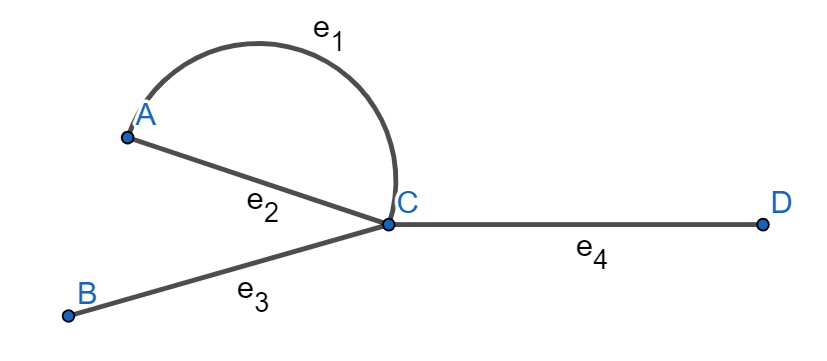
\includegraphics[scale = 0.3]{imgs/graph_nocoop.png}
	\centering
	\caption{Пример графа $G_1$ без некооперативного равновесия}
	\label{fig:nocoop}
\end{figure}

Будем считать, что для длин ребер выполнены следующие неравенства:

$$ l_{e_2} < l_{e_3} < l_{e_1}, \text{ } l_{e_4} > l_{e_3} - l_{e_2}, \text{ } l_{e_4} > l_{e_1} - l_{e_3}. $$

Данные ограничения необходимы для появления следующих ситуация при выборе пути первым участником (см. рис \ref{fig:nocoop_str}):

\begin{figure}[hpt]
	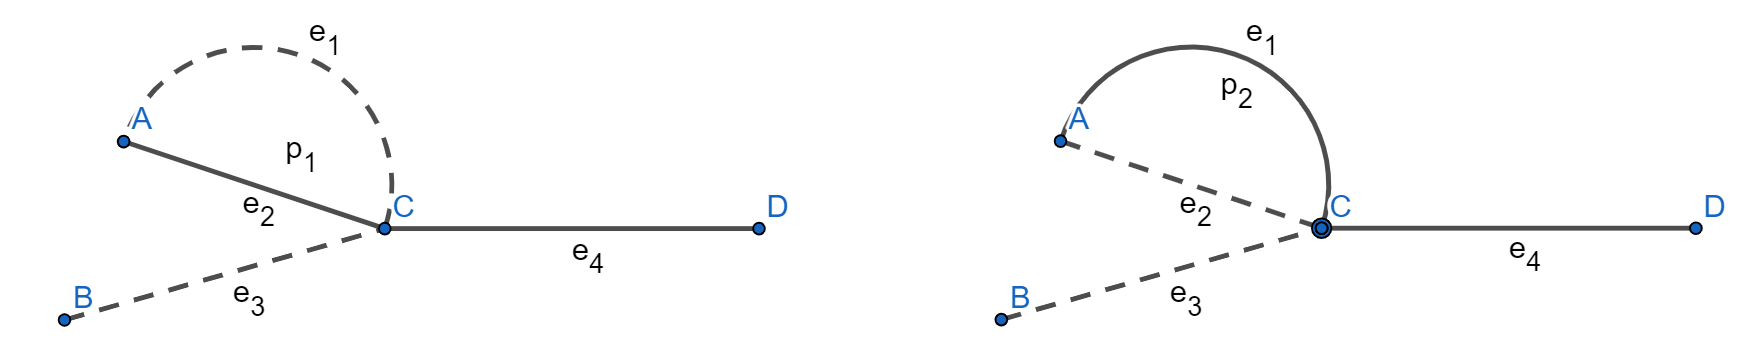
\includegraphics[scale = 0.3]{imgs/no_nocoop_rovn.png}
	\centering
	\caption{Выгодная стратегия участника 1 (слева) и выгодная стратегия участника 2 (справа).}
	\label{fig:nocoop_str}
\end{figure}

При выборе участником 1 пути $p_1 = Ae_2Ce_4D$ 

Для такого графа считаем, что выполнены следующие неравенства.
$$l2 < l3 < l1,$$
$$l4 > $$



\end{document}